\cleardoublepage

\chapter{Dream content}
\label{sec:dream-content}

\cleanchapterquote{Prétendre donner les rêves comme de simples jeux de la pensée, de simples images de l’imagination, c’est témoigner d’un manque de réflexion ou de loyauté ; car de toute évidence ils en diffèrent spécifiquement. Les images de l’imagination sont faibles, languissantes, incomplètes, partielles et si fugitives qu’on peut à peine fixer dans sa mémoire pendant quelques secondes les traits d’un absent, et que même le jeu le plus vif de l’imagination ne peut nullement entrer en comparaison avec la réalité palpable que le rêve met sous nos yeux.\endnote{Free translation to English: \q{To assimilate dreams as mere thoughts or images of the imagination, is to show a lack of reflection or loyalty; because obviously they differ from it specifically. The images of the imagination are feeble, languid, incomplete, partial, and so fleeting that one can scarcely fix in his memory for a few seconds the features of an absent, and that even the most lively play of the imagination cannot be compared to the palpable reality that dreams bring before our eyes.}}}{Schopenhauer}{Parerga und Paralipomena, 1851}

\section{Measuring dream content}
\label{sec:dream-content:method}

Empirical investigation of dreams started in the nineteenth century when scholars started to quantify aspects of their dream content. One notable example is the pioneering paper of Mary Calkins \citeyearpar{calkins_statistics_1893}, entitled \q{Statistics of dreams}, in which she reported, inter alia, statistics concerning dream length and vividness, dream characters and dream-waking-life associations. Since then, a considerable numbers of scales and rating systems for reducing and analyzing dream content have been developed, all based on the assumption that \q{particular aspects of the verbal material ... have to be quantified in order to carry out statistical analyses} \citep{schredl_dream_2010}. Perhaps one of the most famous is the Hall \& Van de Castle coding system \citeyearpar{hall_content_1966}, whose basic idea is to divide dream content into several empirical categories (e.g. settings, objects, characters, interactions, emotions, misfortunes) that can be then used to find patterns and identify prevalent themes among groups of dreamers. The Hall \& Van de Castle coding system remains today the major reference since it has proven stable over at least one generation \citep{hall_dreams_1982}. More recently, \citet{schwartz_exploration_1999} proposed an automatic analysis of the lexical content of dream reports, without any a priori coding of their content, a method which has the advantage of minimizing the experimenter bias and being easily replicable by others.

As pointed out by \citet{schredl_dream_2010}, dream content analysis has several flaws. First, these scales, by reducing dream content to specific dimensions, voluntarily omit a certain amount of the information comprised within the dream report. Second, the results of these scales can drastically differ depending on whether the dream content is self-rated by the dreamer or rated by an external judge. As an example, \citet{sikka_i_2014} recently demonstrated that self-ratings resulted in greater estimates of emotional dreams, and especially positively valenced dreams, that are often found to be a minority when dreams are rated by external judges.

\section{Phenomenology of dreams}
\label{sec:dream-content:pheno}

The empirical analyze of dream content using various scales has allowed to describe several generalizations about the phenomenology of dreams (reviewed in \citealp{hall_content_1966, schwartz_exploration_1999, schredl_characteristics_2010, ruby_experimental_2011, domhoff_finding_2013, windt_dreaming:_2015}). These are detailed as follows:

\begin{my_list_item}
    \item Dreams tend to be negatively valenced
	\item Aggressions are more frequent in dreams than friendly interactions
	\item The visual modality is the predominant sensory modalities in dreams
	\item The dream drama is mostly lived by the dreamer from a first-person perspective
	\item Some elements of real-life events previously experienced by the dreamer often contribute to dream content
	\item Most of the time, the dream sequence is not within the dreamer’s voluntary control
    \item With the exception of lucid dreaming, the dreamer is convinced that the dream's sequence is really happening.
	\item Dream content often contains temporal and spatial inconsistencies
	\item Dream content is often full of people interacting with each other (e.g., discussions, fights, pursuit, sexuality)
	\item Emotions are frequently present during dreams
\end{my_list_item}

\section{Factors influencing dream content}
\label{sec:dream-content:factors}

\citet{de_koninck_sleep_2012} has reviewed in his book entitled \q{Sleep, dreams and dreaming} the factors enabling dream construction, as well as their relative contribution to the dream content. He proposed that the different sources of dreams are best represented in a pyramidal manner, from low levels, predominant in shaping the dream content, to higher levels that carry much less influence to the dream content (Fig \ref{fig:intro:koninck}). A non-exhaustive list of the experimental findings related to each of these \q{layers} of the dream construction is reported in the following paragraphs (see \citealp{blagrove_trait_2010, schredl_characteristics_2010, ruby_experimental_2011, de_koninck_sleep_2012})

\begin{figure}[htb]
	\centering
	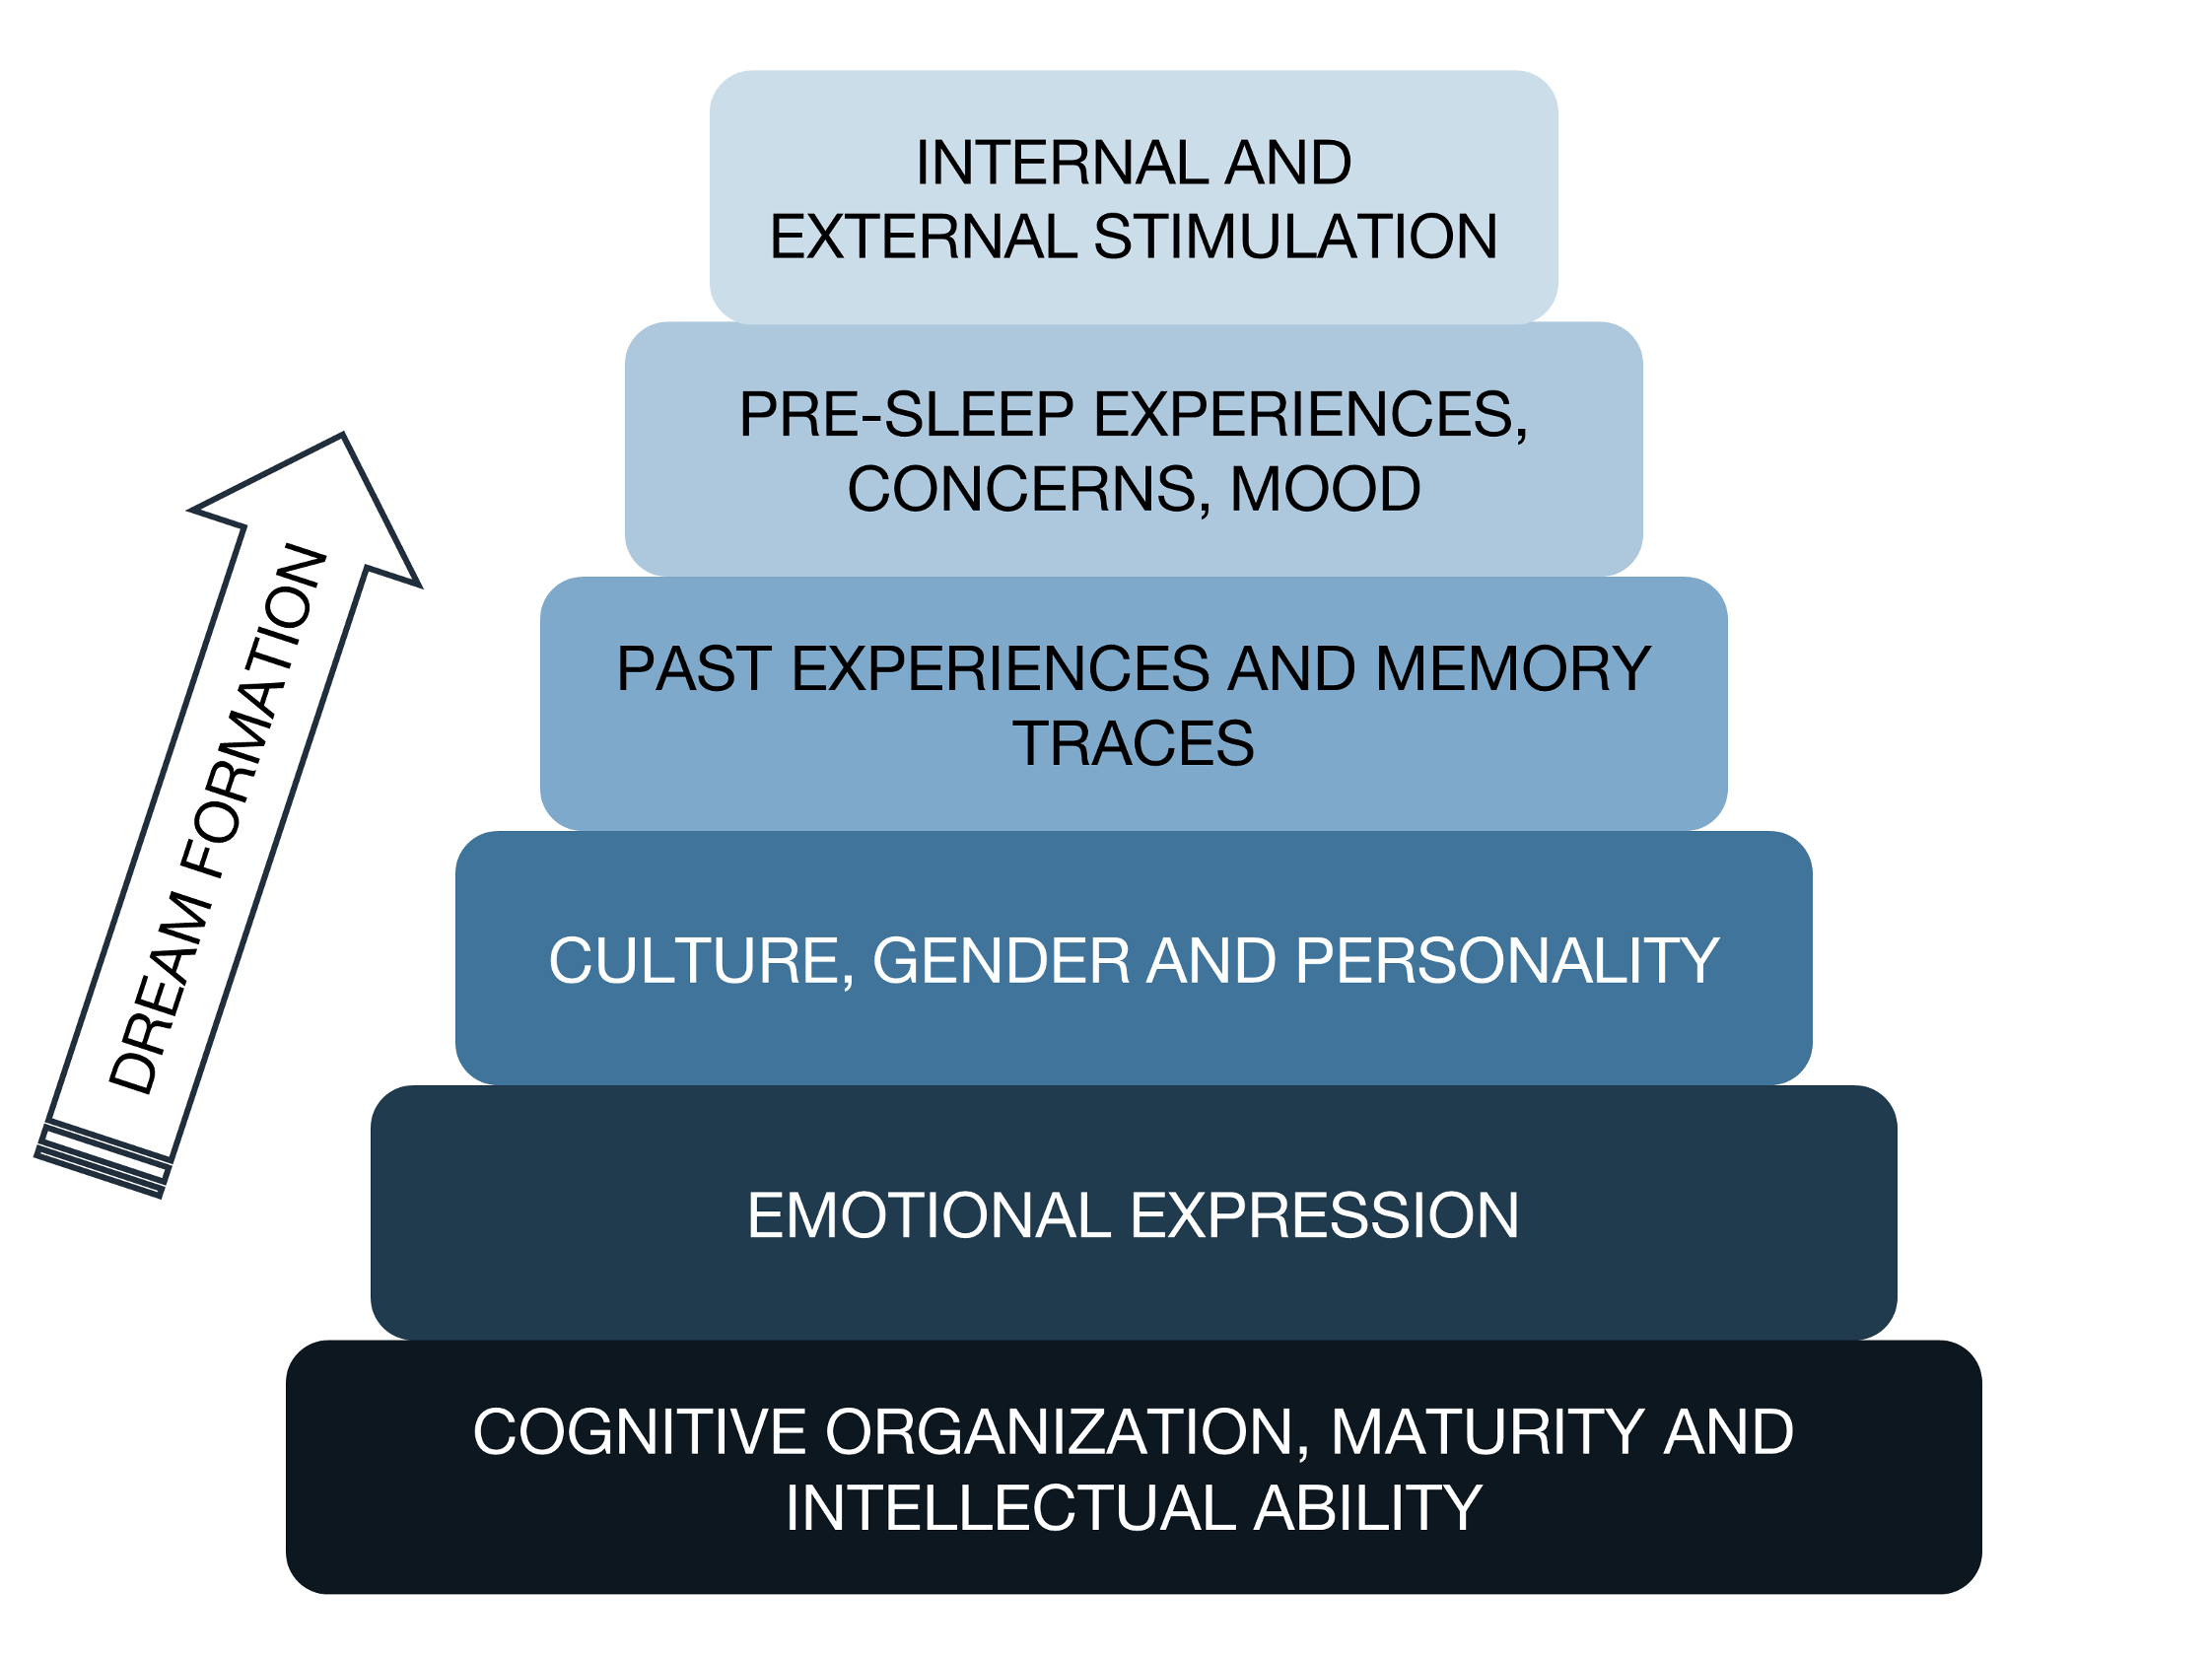
\includegraphics[width=0.8\textwidth]{Fig/Intro/Intro_Pyramid_dream_construction/Intro_pyramid_dream.png}
	\caption[Factors involved in the construction of dreams]{\textbf{Factors involved in the construction of dreams}. The various factors in the elaboration of dreaming are illustrated as a pyramid suggesting their order and importance. Adapted from \citet{de_koninck_sleep_2012}.}
	\label{fig:intro:koninck}
\end{figure}


\paragraph{Cognitive organization, maturity and intellectual ability}

De Koninck's model situates the cognitive organization and capacity as the more crucial determinant in the elaboration of dream content. In line with this, several studies indicated that the cognitive organization of dreams follows the cognitive development of children \citep{foulkes_childrens_1982, foulkes_rem_1990}, and that, similarly, even in adults and elderly, the organization and content of dreams parallels the waking cognitive ability of the dreamer (see \citealp{cavallero_dreaming_1993}). Based on these findings, \citet{domhoff_new_2001} has postulated that \q{dreaming is a cognitive achievement} that depends upon the maturation of forebrain areas.

\paragraph{Emotional expression}

It is now well admitted that waking emotionality is an important contributor to dream formation. Notably, negative emotion seems to prevail in dreams, and can culminate in nightmares or bad dreams \citep{zadra_nightmares_2000, zadra_variety_2006}. This observation led Hartmann to propose that emotions are the primary generator of dream \citep{hartmann_nature_2007, hartmann_central_2008}. According to him, emotions could \q{guide the creation of connections to existing memory systems that in turn lead to new associations that have an adaptive value} \citep{de_koninck_sleep_2012}.

\paragraph{Culture, gender and personality}

Experimental findings suggest that there are both similarities and differences in dream content across culture and societies \citep{domhoff_similarities_2008}. Apparent similarities include dream content seems to be universally more negative than positive (i.e. with a predominance of aggression, misfortune, failure). At the same time, culture-specific differences were observed, for example, in the percentages of animals characters and in the rate of aggressive interactions per character. Gender differences in dream content have been consistently reported, with men reporting more often physical aggression and sex than women \citep{nielsen_typical_2003, schredl_typical_2004}. Personality seems also to influence dream content, and especially moderate the magnitude of continuity between waking and dreaming \citep{schredl_dreaming_1996, schredl_characteristics_2010}.

\paragraph{Past experiences and memory traces}

There is ample evidence that waking experience finds its way into dreams. Many aspects of the subject’s daily life influence dream content, including news event, musical practice, current concerns and religious beliefs, chronic pain, mood or living in a violent environment (see \citealp{ruby_experimental_2011}). This observation has led to the so-called \q{continuity hypothesis of dreaming} which simply states that dreams reflect waking life experiences \citep{schredl_continuity_2003}. However, the characteristics and time course of the waking memory sources integrated into dreams are still unclear. Furthermore, there is a rising consensus that dream content very rarely replays an episodic memory exactly as it was originally experienced \citep{fosse_dreaming_2003, nielsen_what_2005}.

Several factors have been positively associated with the likelihood of a waking life experience to be incorporated into dreams (reviewed in \citealp{schredl_characteristics_2010}). First, there seems to be a linear decrease in temporal references identified in dreams (i.e. recent experiences are more incorporated into dreams than older ones \citealp{botman_dream_1990, strauch_dem_2004, grenier_temporal_2005}), an observation supporting the notion of continuity between waking and dreaming memory processes. However, and contrarily to what would be expected according to this memory decay with time, some studies reported an overrepresentation in dreams of waking experiences that happened approximately one week before the dream \citep{nielsen_day-residue_1992, marquardt_empirical_1996, blagrove_replication_2011}. This so-called \q{dream-lag effect} was however not consistently found and seems to be specific to REM dreams \citep{blagrove_assessing_2011, van_rijn_dream-lag_2015}. Second, all waking life activities are not represented in the same proportion in dreams \citep{hartmann_we_1996, schredl_continuity_2000}. Focused thinking activity (e.g. using a computer or reading) occurs less frequently than unfocused activities such as talking with friends. Third, several studies reported a preferential incorporation of emotional waking-life experiences into dreams \citep{malinowski_evidence_2014, schredl_factors_2006}. Interestingly, these authors reported that emotional intensity, but not emotional tone, seems to affect the incorporation into subsequent dreams.

\paragraph{Pre-sleep experiences, concerns, mood}

Several studies \citep{botman_dream_1990, nielsen_day-residue_1992, marquardt_empirical_1996} have confirmed that a significant proportion of dreams contain elements that refer to experiences of the preceding day, a phenomenon known as day-residues and mentioned by Freud who considered them as \q{a necessary ingredient in dream formation} \citep{freud_interpretation_1900}. Interestingly, the incorporation of pre-sleep experiences seems to be influenced by chronobiological factors, such as sleep cycles and time of the night. For example, dream reports from the first part of the night comprise more day-residues than dream reports from the second part of the night, which contain more elements from the distant past \citep{roffwarg_effects_1978}.
Current concerns and pre-sleep mood also influence dream content. Studying dream content and concerns over a period of 5 months in depressed and controls subjects who were all going through a divorce, \citet{cartwright_relation_2006} remarkably found that the degree of waking concern about the ex-spouse was significantly correlated with the number of dreams in which the former partner appeared as a dream character. Furthermore, she reported that not only dream content is related to the ongoing emotional concerns of the dreamer, it seems \emph{per se} to play an active role in the down-regulation of disturbed mood (see section \ref{sec:dream-func:modern:emotion}, \citealp{cartwright_dreams_1991, cartwright_role_1998, cartwright_role_1998, cartwright_relation_2006}).

\paragraph{External and internal stimulation}

\q{From this it is manifest that the stimulatory movements based upon sensory impressions, whether the latter are derived from external objects or from causes within the body, present themselves not only when persons are awake, but also then, when this affection which is called sleep has come upon them, with even greater impressiveness} (Aristotle, On Dreams, 350 B.C.E). More than two thousand years ago after Aristotle's famous essay, experimental studies have confirmed that external stimulation can be incorporated into dream content. For instance, as we mentioned earlier in section \ref{sec:dream-research:link:goblot}, \citet{dement_relation_1958} have reported an incorporation of non-awakening water stimulations in 42\% of the subsequent dream reports. Such incorporation of external stimuli into dreams also inspired the famous Dali painting \emph{Dream Caused by the Flight of a Bee Around a Pomegranate a Second Before Awakening}.
